\section{Genetic Algorithms}
In this section we begin with a brief overview of the standard implementation of a Genetic Algorithm (GA) and include
pseudocode for the readers reference. Next, we discuss our implementation and the design choices made so we could easily
use our implementation for two different problems. We then look at one of these problems and highlight how a GA is an
appropriate choice. This also serves to provide the reader with an example of how a GA can be applied in practice.
Finally, we discuss the challenges faced in using the GA to solve this particular problem.


\subsection{Overview, Design and Intention}
Algorithm \ref{GA_alg} is our implementation of the standard GA. Methods such as \textbf{SelectParent()}, \textbf{CrossOver()}, \textbf{Mutate()} and \textbf{CalculateFitness()} are abstract and implemented by the subclass.
In doing this, it was trivial to use the GA for two different problems. Additionally, it allowed us to experiment with 
different selection methods, such as proportional roulette, tournament and ranked roulette by simply 
overriding \textbf{SelectParent()}. Similarly, the same can be said for crossover and mutation.
\begin{algorithm}[h]
\begin{algorithmic}
\State $children \gets$ InitEmptyPopulation()
\State $numChildren \gets 0$ 
\ForAll{$members$ in $population$} 
	\State $fitness[member] \gets$ CalculateFitness($member$)
\EndFor

\While{$numChildren < populationSize$}
	\State $parent1 \gets$ SelectParent()
	\State $parent2 \gets$ SelectParent()
	\If{$randomVal < crossoverRate$}
		\State $child1$, $child2 \gets $ CrossOver($parent1$, $parent2$)
	\Else
		\State $child1$, $child2 \gets $ Copy($parent1$, $parent2$)
	\EndIf
	\State Mutate($child1$) \Comment{\parbox[t]{.75\linewidth}{Where the mutate method handles which genes of the 
	chromosome get mutated according to the mutation rate.}}
	\State Mutate($child2$) 
	\State $children \gets children + child1$
	\State $children \gets children + child2$
	\State $numChildren \gets numChildren + 2$
\EndWhile
\State $population \gets children$ 
\caption{A standard Genetic Algorithm}
\label{GA_alg}
\end{algorithmic}
\end{algorithm}

We employ the use of GA's in our work and believe they are strongly applicable for the following reasons:
\begin{itemize}
\item Many solutions exist in the state space which would be infeasible to manually explore. By defining a fitness function
which encapsulates the properties of a desired solution, we can explore far more possibilities.
\item We can observe solutions which we may never have previously considered.
\item A GA framework is extensible and allows code reuse as the core algorithm can be used for different problems with 
minor changes.
\end{itemize}

\subsection{Tree Placement}
For a player to maximize the amount of resources they collect, a certain subsection of the map
may be far more profitable than another. However, in order to know this they must discover it. If the map topology
remained static, the player would always head to the most profitable area without much pause for thought.
In order to make subsequent games more interesting and enjoyable, we decided to randomize the placement of
the resource trees. 

The objective of the GA and fitness function was to optimize the placement of dynamic objects around the borders
of the map at the start of the game. 
We chose tournament selection as it can reach a local optimal solution in a smaller number of 
iterations and for our problem, we do not require the exact solution, an approximate one will do (the time cost 
of ranked roulette isn't worth it).
\begin{figure}[h]
        \centering
        \begin{subfigure}[b]{0.482\linewidth}
                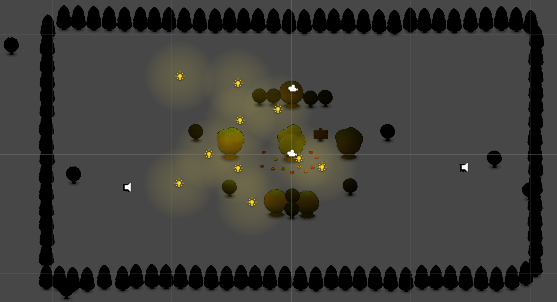
\includegraphics[width=\linewidth]{./ga_n1}
                \caption{}
                \label{fig:ga_step1}
        \end{subfigure}
        \begin{subfigure}[b]{0.49\linewidth}
                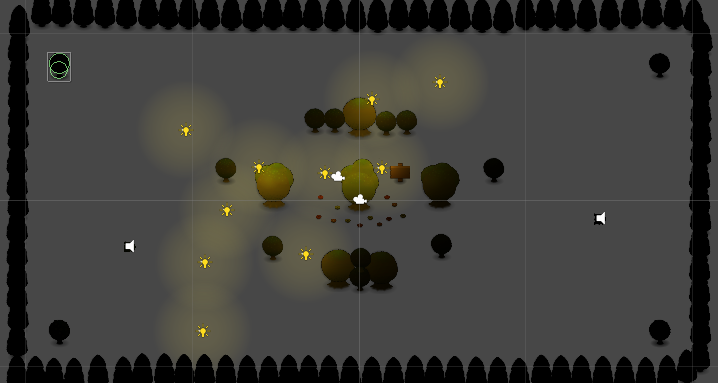
\includegraphics[width=\linewidth]{./ga_n2}
                \caption{}
                \label{fig:ga_step2}
        \end{subfigure}
        \begin{subfigure}[b]{0.5\linewidth}
                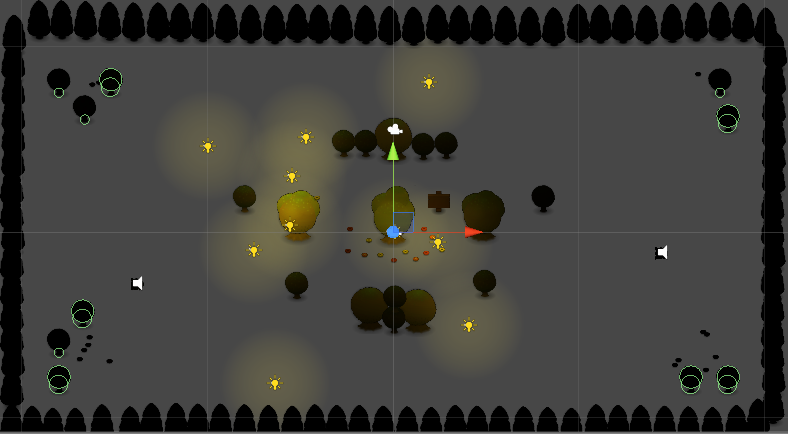
\includegraphics[width=\linewidth]{./ga_n3}
                \caption{}
                \label{fig:ga_step3}
        \end{subfigure}
        \begin{subfigure}[b]{0.49\linewidth}
               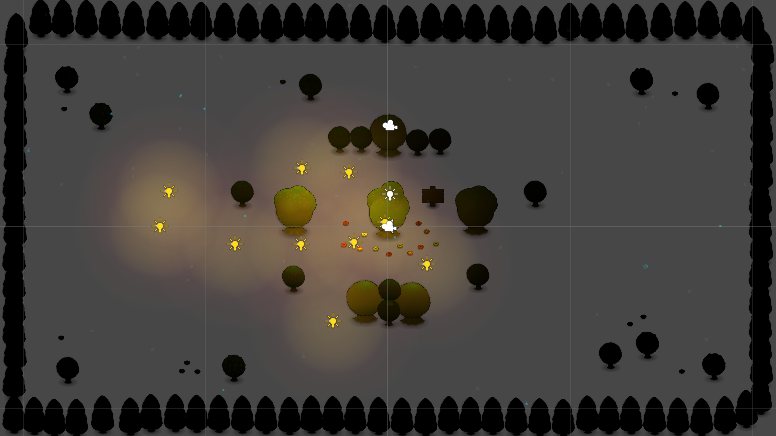
\includegraphics[width=\linewidth]{./ga_final}
           	   \caption{}
               \label{fig:ga_step4}
        \end{subfigure}
        \caption{The steps to implementing an appropriate fitness function. In \ref{fig:ga_step1} the trees are placed 
        outside of the game border. If we left the GA to run for 100,000 iterations, the trees were much further away and 
        to see them the scene must be zoomed out. In \ref{fig:ga_step2} we remedied this problem , yet created a new one. 
        Here the trees remained in the four corners of the map as the GA found an optimal solution which maximised this 
        fitness function. To prevent this behaviour, we needed to take the distance to other gameobjects into consideration which adds some extra overhead. Figure \ref{fig:ga_step3} shows 
        the inclusion of flower positions. As one can see there is quite a lot which are clustered. Removing the number of flowers generated did not solve this issue. Instead, the fitness function needed minor alterations in regards to the required distance a gameobject should be from another. Figure 
        \ref{fig:ga_step4} shows the final fitness function and GA parameter set. Here the flowers and trees are spread out 
        far more. Additionally, this iteration of the GA gives a better amount of randomization on subsequent 
        runs.}
        \label{fig:GA_Trees}
\end{figure}


\subsection{Challenges}
In this section we highlight the challenges we faced for the specific problem of randomizing
the placement of objects in the game world. We leave discussion of the challenges related to evolving weights
for a neural net to train a frog controller for section \ref{sec:neuro}.

\subsubsection{Tournament Selection}
A minor issue we faced with tournament selection was that it was initially selecting too many
chromsomes with a low fitness value to breed children for subsequent populations. The inital tournament
size was 2 and when randomly selecting chromosomes to take part in such a small tournament, the majority of the 
population was being filled with poor solutions. We changed the tournament size to be half of the total 
population and witnessed immense improvements in the solutions that were being generated, as the chromsomes with 
a low fitness value were unlikely to be present or have offspring in the next population.

\subsubsection{Fitness Function and Parameters}
Briefly, we note the common issue that the fitness function and parameters of a GA often requires a 
substantial amount of experimentation and tweaking. Situations which you 
previously did not take into consideration may arise in generated solutions and you thus need to account for 
them. Additionally, one must balance the positive and negative costs. For example, in Figure \ref{fig:ga_step1}
our original fitness function did take into consideration that chromosomes with tree positions outside the 
boundaries should have a lower fitness. However, as the fitness was calculated as the cumulative distance
of the tree to other trees, as the trees got further and further away, the fitness value was always higher
than the penalty for being outside the boundary. We discuss how we solved such issues in Section 
\ref{sec:runtimeIssues}, here we simply point out the common issues with GA's in general and there
reliance on an appropriate fitness function and parameters.

\subsubsection{Generating Positions at Runtime} \label{sec:runtimeIssues}
One of the issues we faced was generating the positions for the flowers and trees at runtime. Here we did not
have the luxury of running the algorithm offline and then plugging in the result later. Therefore,
we had to get the right balance of parameters (number of trees/flowers, epochs, crossover rate, mutation rate 
and mutation amount) to generate the solution in an acceptable time frame. We found that running for less epochs 
wasn't too much of an issue as it gives us a better random selection of map layouts. However, in some
rare circumstances, trees/flowers may overlap or be placed in the middle of the lake with a poor initial
population.

The problem was further exaggerated by the fact that there was objects which were already statically placed on 
the map. In this instance, we could solve this simply by placing an invisible boundary around the center
game objects, which if a resource tree was placed inside, the fitness would be heavily worsened. Additionally,
in an attempt to speed up generating an acceptable solution, we check for the following:
\begin{itemize}
\item Overlapping trees/flowers
\item Trees/Flowers outside boundaries of map
\item Trees/Flowers in the lake
\end{itemize}
and if they exist, assign a fitness of 0 as we never want them to occur. Therefore, during selection, there is
a very low probability that they will see future generations.

\subsection{Outcome}
Figure \ref{fig:GA_Final} shows several different solutions generated by the final fitness functions and 
parameter set (Table \ref{table:params}).
It's interesting to note the variations in each. Lastly, Figure \ref{fig:fitnessOverTime} shows
how the largest individual fitness value changes over the course of 1500 epochs.

\begin{table}[h]
	\centering
    \begin{tabular}{ | l | l |}
    \hline
    Parameter & Setting \\ \hline
    Mutation Rate & 0.001    \\ \hline
    Crossover Rate & 0.7    \\ \hline
    Vector Mutate (i.e. vec.x or vec.y $\pm$ vector mutate) & 1.5    \\ \hline
    Epochs & 1500    \\ \hline
    Number of Trees & 8    \\ \hline
    Number of Flowers & 10    \\ \hline
    \end{tabular}
    \caption{Final parameter settings for object placement.}
    \label{table:params}
\end{table}

\begin{figure}[h]
\centering
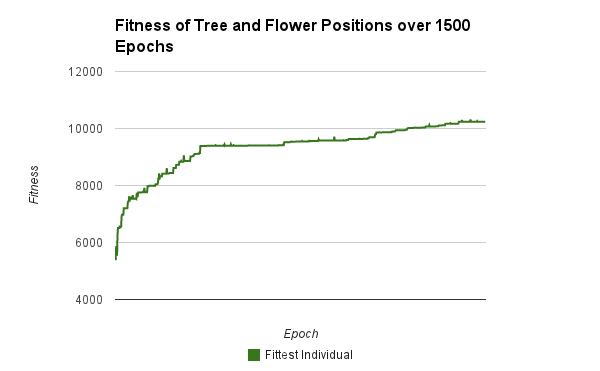
\includegraphics[width=0.7\linewidth]{./timeFitness}
\caption{Fitness of the fittest individual over 1500 Epochs.}
\label{fig:fitnessOverTime}
\end{figure}

\begin{figure}[h]
        \centering
        \begin{subfigure}[b]{0.48\linewidth}
                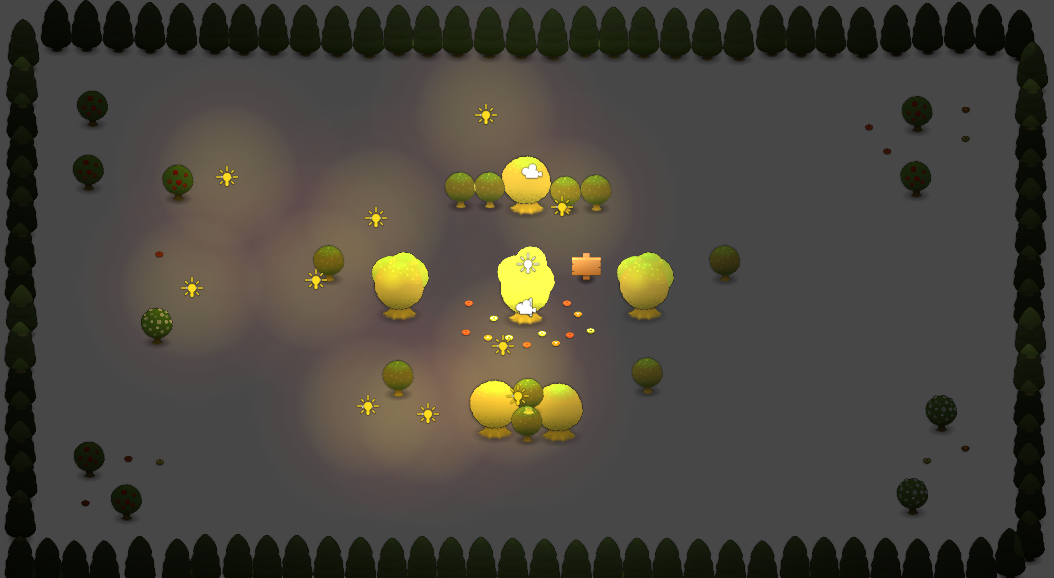
\includegraphics[width=\linewidth]{./ga_outcome_1}
                \caption{}
                \label{fig:ga_outcome_1}
        \end{subfigure}
        \begin{subfigure}[b]{0.48\linewidth}
                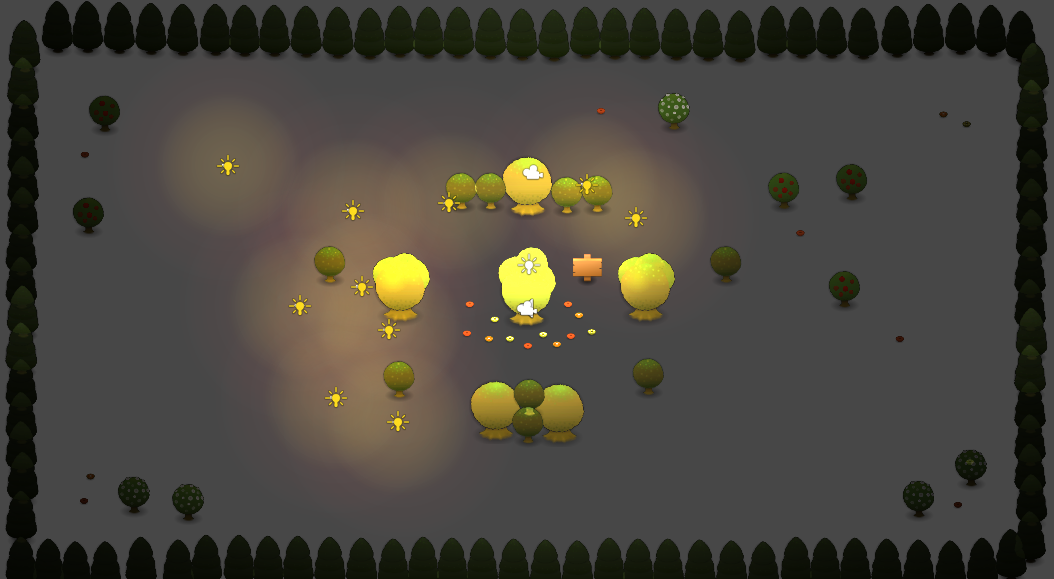
\includegraphics[width=\linewidth]{./ga_outcome_2}
                \caption{}
                \label{fig:ga_outcome_2}
        \end{subfigure}
        \begin{subfigure}[b]{0.48\linewidth}
                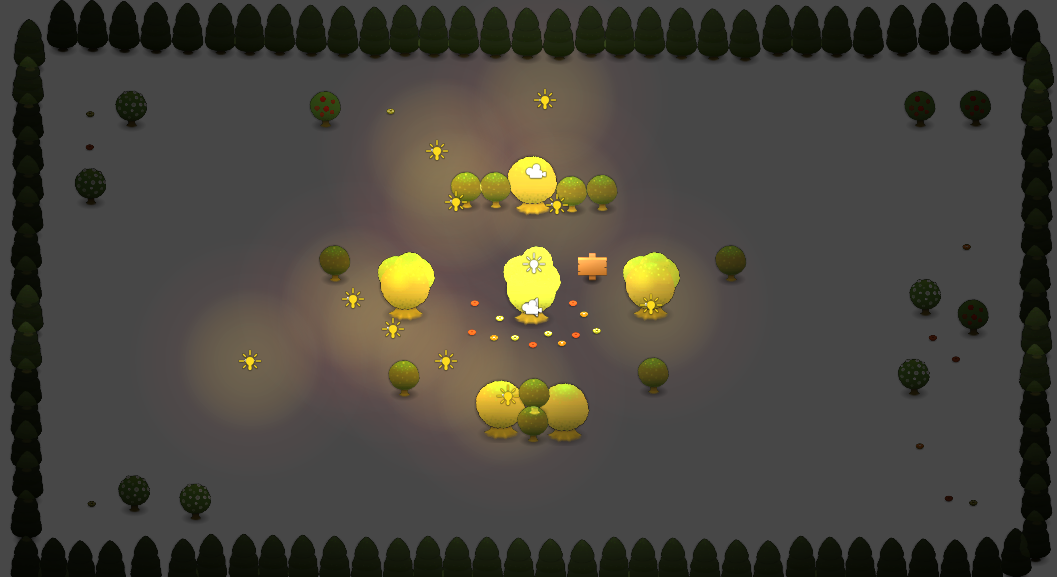
\includegraphics[width=\linewidth]{./ga_outcome_3}
                \caption{}
                \label{fig:ga_outcome_3}
        \end{subfigure}
        \begin{subfigure}[b]{0.48\linewidth}
                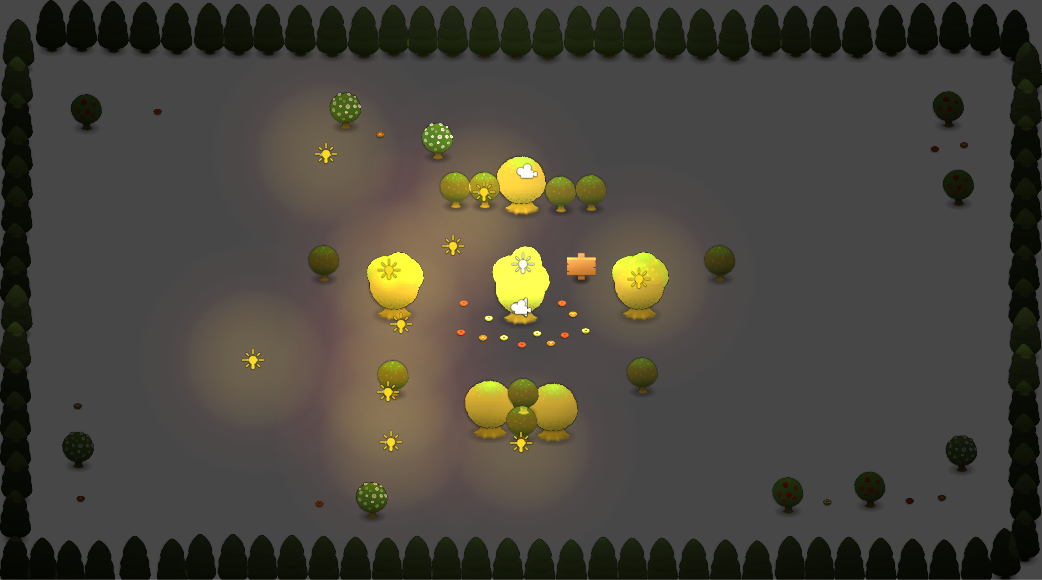
\includegraphics[width=\linewidth]{./ga_outcome_4}
                \caption{}
                \label{fig:ga_outcome_4}
        \end{subfigure}
        \begin{subfigure}[b]{0.48\linewidth}
                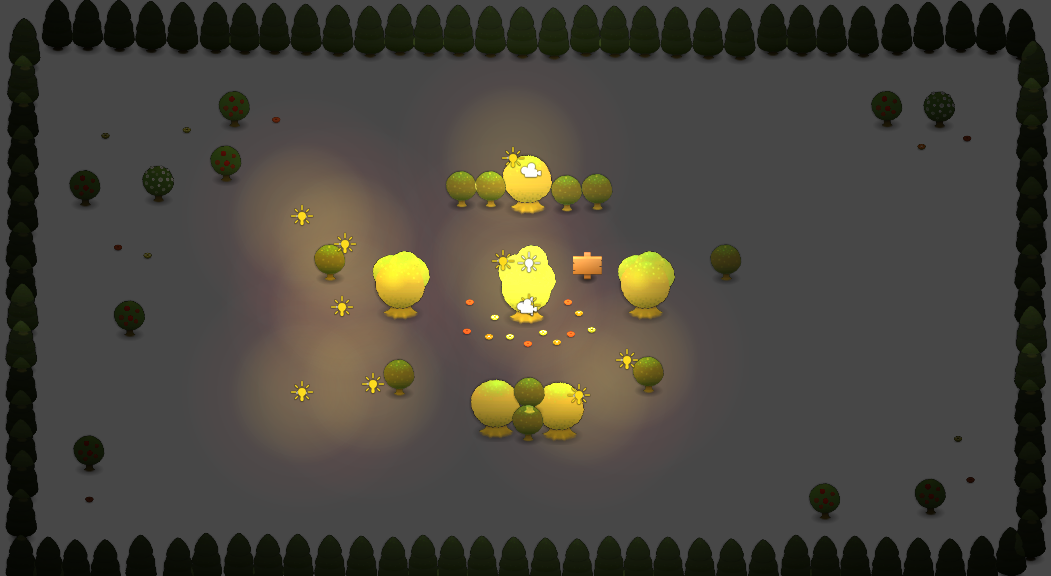
\includegraphics[width=\linewidth]{./ga_outcome_5}
                \caption{}
                \label{fig:ga_outcome_5}
        \end{subfigure}
        \begin{subfigure}[b]{0.48\linewidth}
                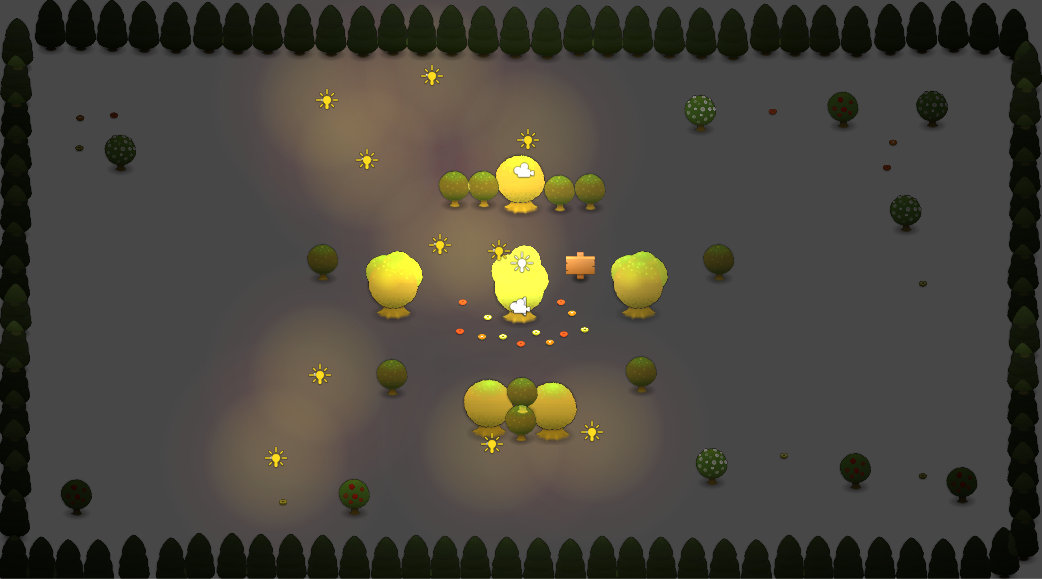
\includegraphics[width=\linewidth]{./ga_outcome_6}
                \caption{}
                \label{fig:ga_outcome_6}
        \end{subfigure}
        \caption{A subset of solutions generated by the final fitness function and parameter set.}
        \label{fig:GA_Final}
\end{figure}